% !TEX root= ../main.tex
\section{Odd paths}
\label{sec:Odd paths}
We already know that whenever two vertices are connected by an edge, like the two vertices in the graph below\footnote{Dashed lines will represent possible edges to irrelevant parts of the graph.  If a vertex has no dashed edges, it means that we disallow it}, their binary NAND is provable in Neg.
\[
  \begin{tikzpicture}
    [
    node distance=1.5cm,
    point/.style={circle,draw,inner sep=0pt,minimum size=2mm},
    ]
    \node (1) at (1,1) [point] {};
    \node (2) at (2,1) [point] {};
    \draw [-latex] (1) to (2);

    \node (e1) [above left=4mm and 6mm of 1]  {};
    \node (e2) [left=8mm of 1] {};
    \node (e3) [below left=4mm and 6mm of 1] {};
    \node (e4) [above right=4mm and 6mm of 2] {};
    \node (e5) [right=8mm of 2] {};
    \node (e6) [below right=4mm and 6mm of 2] {};
    \draw [dashed] (e1) to (1);
    \draw [dashed] (e2) to (1);
    \draw [dashed] (e3) to (1);
    \draw [dashed] (e4) to (2);
    \draw [dashed] (e5) to (2);
    \draw [dashed] (e6) to (2);
  \end{tikzpicture}
\]
It is however easy to find a case examplifying how the implication does not hold in the opposite direction.
\[
  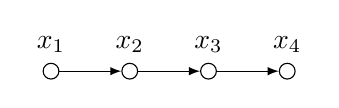
\begin{tikzpicture}
    [
    point/.style={circle,draw,inner sep=0pt,minimum size=2mm},
    ]
    \node (1) at (0,1) [point,label=above:$x_1$] {};
    \node (2) at (1,1) [point,label=above:$x_2$] {};
    \node (3) at (2,1) [point,label=above:$x_3$] {};
    \node (4) at (3,1) [point,label=above:$x_4$] {};
    \draw [-latex] (1) to (2);
    \draw [-latex] (2) to (3);
    \draw [-latex] (3) to (4);
  \end{tikzpicture}
\]
The vertices $x_1$ and $x_4$ in the above graph are not connected by an edge, but by a path.
The NAND-clause $\ol{x_1x_4}$ is however still easily proved in Neg.
\begin{prooftree*}
  \Hypo{\ol{x_1x_2}}
  \Hypo{\ol{x_3x_4}}
  \Infer[left label=$x_2x_3$]2{\ol{x_1x_4}}
\end{prooftree*}
Making the path between two vertices longer does not affect the provability of the corresponding binary NAND.
Consider the below graph.
\[
  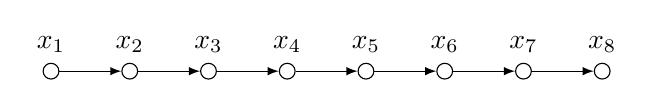
\begin{tikzpicture}
    [
    point/.style={circle,draw,inner sep=0pt,minimum size=2mm},
    ]
    \node (1) at (0,1) [point,label=above:$x_1$] {};
    \node (2) at (1,1) [point,label=above:$x_2$] {};
    \node (3) at (2,1) [point,label=above:$x_3$] {};
    \node (4) at (3,1) [point,label=above:$x_4$] {};
    \node (5) at (4,1) [point,label=above:$x_5$] {};
    \node (6) at (5,1) [point,label=above:$x_6$] {};
    \node (7) at (6,1) [point,label=above:$x_7$] {};
    \node (8) at (7,1) [point,label=above:$x_8$] {};
    \draw [-latex] (1) to (2);
    \draw [-latex] (2) to (3);
    \draw [-latex] (3) to (4);
    \draw [-latex] (4) to (5);
    \draw [-latex] (5) to (6);
    \draw [-latex] (6) to (7);
    \draw [-latex] (7) to (8);
  \end{tikzpicture}
\]
$\ol{x_1x_8}$ can be proven in Neg in the following way:
\begin{prooftree*}
  \Hypo{\ol{x_1x_2}}
  \Hypo{\ol{x_3x_4}}
  \Infer[left label=$x_2x_3$]2{\ol{x_1x_4}}
  \Hypo{\ol{x_5x_6}}
  \Infer[left label=$x_4x_5$]2{\ol{x_1x_6}}
  \Hypo{\ol{x_7x_8}}
  \Infer[left label=$x_6x_7$]2{\ol{x_1x_8}}
\end{prooftree*}
More generally, whenever two vertices are connected by a path of odd length, their corresponding NAND-clause is provable.
